% Narrative revision, 15 October 2026.
% Source of record: accentuation_rmt_main_compact_draft.tex -> main_body_compact.tex.
% COSYNE rules verified at https://www.cosyne.org/abstracts-submission.
% 12 pt body, A4, 0.55 in margins; 10 pt captions/references; anonymous.
% A/B reuse existing result panels; C replots reported correlations.
% Regenerate the figure with python3 notes/build_cosyne2027_figure.py.
\documentclass[12pt,a4paper]{article}
\usepackage[margin=0.55in]{geometry}
\usepackage[T1]{fontenc}
\usepackage{times,amsmath,amssymb,graphicx,caption}
\usepackage[hidelinks]{hyperref}
\hypersetup{pdftitle={Why accurate neural predictions do not guarantee effective neural control},pdfauthor={},pdfsubject={COSYNE 2027 extended abstract},pdfkeywords={}}
\pagestyle{empty}
\setlength{\parindent}{0pt}
\setlength{\parskip}{5pt}
\setlength{\abovedisplayskip}{5pt}
\setlength{\belowdisplayskip}{5pt}
\setlength{\emergencystretch}{1.5em}
\captionsetup{font=footnotesize,labelfont=bf,labelsep=period,skip=4pt,hypcap=false}
\newcommand{\head}[1]{\par\noindent\textbf{#1}\enspace\ignorespaces}
\newcommand{\bh}{\hat\beta}
\newcommand{\bt}{\beta^\star}
\newcommand{\mb}{\bar\beta}
\begin{document}
{\large\bfseries Why accurate neural predictions do not guarantee effective neural control\par}

\textbf{Summary.}
Encoding models of visual cortex are increasingly used to design images that drive neurons toward a chosen response. Yet models with similar accuracy on natural images can differ sharply in how well their generated images control neural activity. Why does successful prediction fail to transfer to control? We develop a regression theory motivated by a closed-loop comparison of ten models at 25 recording sites in five macaques. The central distinction is which inputs evaluate the model: prediction uses natural images, whereas control follows a direction chosen by the model itself. Natural images constrain some directions strongly and others weakly. Errors in the weakly constrained directions can therefore have little effect on prediction while dominating stimulus optimization. In a linear model, random matrix theory quantifies how finite data and noisy responses create these errors, and shows why regularization selected for prediction need not prevent control failure. Extending the theory to fixed feature maps, we construct models with identical predictive performance but sharply different control, isolating a gradient-geometry factor that prediction scores do not determine. A corresponding diagnostic for deep networks is associated with biological control across the models in the motivating experiment, whereas held-out prediction error is largely uninformative. The theory also explains how a model can recognize effective stimuli generated by another model while failing to generate them itself. These results identify a limit of prediction-based model evaluation and motivate testing gradient geometry or generated stimuli when selecting models for neural control.

\head{Additional detail: the experimental puzzle.}
Prince, Wang, et al.~[1] fitted deep-network encoding models to naturalistic-image responses from macaque V3/V4, inferotemporal cortex and superior temporal sulcus. Each model then modified seed images to reach graded predicted response targets, using feature accentuation~[2]; the images were presented to the same neural sites. Across nine trained models and an untrained baseline, prediction and control gave different rankings. The trained models had similar natural-image predictivity, but their control stimuli differed visibly and often added high-frequency structure with little effect on the neuron. Some unsuccessful controllers nevertheless predicted responses to a successful model's images. We ask how fitting a model can produce this combination.

\head{Prediction and control test different directions.}
We first model the neuron as a linear teacher, $y=x^\top\bt+\sigma\epsilon$, with Gaussian inputs $x\sim\mathcal N(0,\Sigma)$ and independent unit-variance noise $\epsilon$. A student $f(x)=x^\top\bh$ is fitted by ridge regression to $n$ examples. From a centered seed, gradient ascent follows $x=\alpha\bh$. Along this path the model predicts $\alpha\|\bh\|^2$, while the neuron responds with noiseless mean $\alpha\bh^\top\bt$. Thus
\begin{equation}
E_{\rm gen}=(\bh-\bt)^\top\Sigma(\bh-\bt),
\qquad
\mathrm{slope}_{\rm control}=\frac{\bh^\top\bt}{\|\bh\|^2}.
\label{eq:geometry}
\end{equation}
Here the slope is measured response regressed on model prediction; $\mathrm{slope}=1$ indicates correct calibration. Prediction downweights errors along low-variance image directions. Control instead follows the fitted weight, so these errors can absorb much of the predicted response change without driving the neuron. This mechanism already reproduces the qualitative experimental dissociation without nonlinear features.

\head{Why cross-validation does not remove the problem.}
Using random matrix theory~[3], we derive leading approximations for typical ridge fits in the proportional-limit of dimension and sample size. The mean fitted weight $\mb$ is the teacher shrunk along each covariance eigenvector.%, with effective regularization $\kappa$ 
Finite sampling and response noise add fluctuations around this mean, increasing the fitted weight's squared norm by an amount $V$. At leading order,
\begin{equation}\small
\mathrm{slope}_{\rm control}\simeq
\frac{\mb^\top\bt}{\|\mb\|^2+V},
\qquad
V=\frac{E_{\rm gen}+\sigma^2}{n}
\sum_k\frac{s_k}{(s_k+\kappa)^2},
\label{eq:inflation}
\end{equation}
where $s_k$ are input-covariance eigenvalues and $\kappa$ is the effective ridge penalty accounting for finite sampling. The extra norm increases the model's predicted modulation of the neuron without increasing its actual alignment with the neuron. Once it outweighs shrinkage, the model overpredicts its modulation. 
We derive distinct spectral conditions for prediction-optimal and control-calibrated regularization: their optima generally differ for anisotropic inputs and a structured teacher. Natural-image simulations confirm that cross-validation can retain good prediction while control deteriorates (Fig.~1A).

\newpage
\head{Why equally predictive feature maps control differently.}
To study effect of feature backbones, we fit ridge readouts on fixed linear features $Fx$, giving pixel gradients $\bh=F^\top\hat w$. Prediction depends on the feature covariance $F\Sigma F^\top$ and its relationship to the teacher; control also depends on how features map back into pixels $FF^\top$. We construct transformations preserving the joint feature--response distribution, hence the predicted generalization curve and its optimal penalty stay invariant, while control changes (Fig.~1B). The dissociation can become arbitrarily severe for anisotropic input.

The additional geometry enters the norm inflation through
\begin{equation}\small
V_F=\frac{E_{\rm gen}+\sigma^2}{n}\,T_F(\kappa),
\qquad
T_F(\kappa)=\sum_{k:s_k>0}
\left(\frac{s_k}{s_k+\kappa}\right)^2
\frac{\|g_k\|^2}{g_k^\top\Sigma g_k},
\label{eq:features}
\end{equation}
where $(s_k,v_k)$ now denote feature-covariance eigenpairs and $g_k=F^\top v_k$ is a feature direction's pixel gradient. The sum weights features that survive regularization and compares their gradient energy with natural-image variation along that gradient. Control is fragile when well-estimated features send their gradients into weakly constrained pixel directions, making $T_F$ large without unchanging prediction error.

\head{From linear theory to biological control.}
For nonlinear features $\phi$, we retain the spectral weights $s_k/(s_k+\kappa)^2$ and measure squared pixel-gradient norms $\|J_\phi(x)^\top v_k\|^2$. Their weighted sum, averaged over ten seed images, gives $T_\phi$, a diagnostic computable from a feature backbone before a control experiment. Across nine trained models at 25 sites (225 site--model pairs), $\log_{10}T_\phi$ correlates with site-centered control slope at $r=-0.61$, compared with $r=0.02$ for log held-out mean squared error (Fig.~1C). This supports our heuristic nonlinear extension as a prognostic predictor of control success. %This association weakens substantially without the two adversarially trained models. It supports the diagnostic descriptively; the nonlinear extension is not a proved control-error formula.

\begin{center}
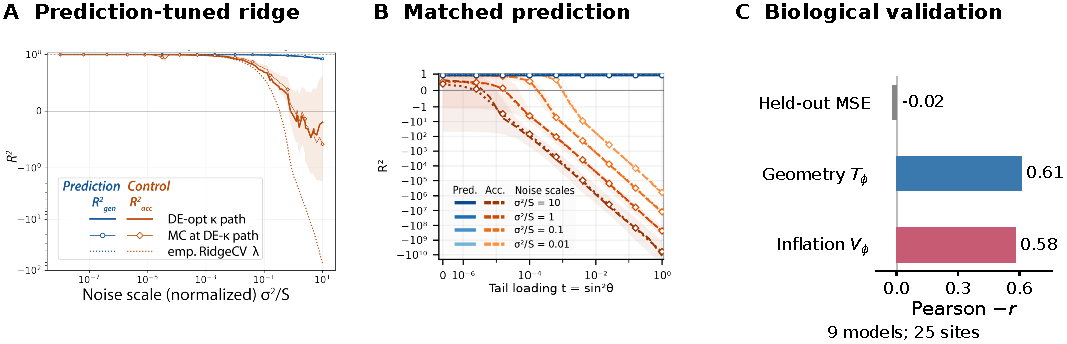
\includegraphics[width=\linewidth]{figures/cosyne2027_v4_evidence.pdf}
\captionof{figure}{\textbf{Three tests of the theory.}
\textbf{A}~Natural-image ridge ($d=10^4$, $n=10^3$): prediction stays good while control $R^2$ becomes negative. Lines: theory; markers/band: Monte Carlo; dotted: empirical cross-validation.
\textbf{B}~Feature rotations preserve prediction (blue) but impair control (orange); shades denote noise levels.
\textbf{C}~Reported correlations of log predictors with site-centered control slope, across nine trained models and 25 sites. $V_\phi=E_{\rm val}T_\phi/n$ includes held-out error and sample size. These are descriptive correlations; no independent-pair significance is assumed.}
\end{center}

\head{Recognition without generation.}
On a peer's path, evaluation depends on a cross-product of weights rather than the evaluator's squared norm. For independent ridge fits, uncorrelated fluctuations remove the leading self-noise inflation, explaining how a poor generator can evaluate another model's images. Shared recordings require accounting for correlated fluctuations. The formal theory assumes linear teachers and fixed linear features, but its practical message extends to encoding-model evaluation: prediction alone cannot certify control. Models must also be tested on the directions or stimuli their optimization will use.

\vspace{2pt}
{\fontsize{10}{11}\selectfont
\textbf{References.}
[1] Prince, Wang, et al. (2026). Parametric neural control differentiates top neural network models of primate visual cortex. \emph{bioRxiv}, doi:10.64898/2026.08.16.745063.
[2] Hamblin et al. (2024). Feature accentuation: Revealing `what' features respond to in natural images. arXiv:2402.10039.
[3] Dobriban \& Wager (2018). High-dimensional asymptotics of prediction: Ridge regression and classification. \emph{Annals of Statistics} 46:247--279.
\par}
\end{document}
